%&tex

\documentclass[usenames,dvipsnames]{beamer}

\usepackage[english]{babel}
\usepackage[utf8]{inputenc}
\usepackage{mathtools}
\usepackage{amsthm}
\usepackage{amssymb}
\usepackage{thmtools,thm-restate}
\usepackage{amsfonts}
\usepackage{hyperref}
\usepackage[singlelinecheck=false]{caption}
\usepackage[backend=biber,url=true,doi=true,eprint=false,style=authoryear]{biblatex}
\usepackage{algorithm}
\usepackage[noend]{algpseudocode}
\usepackage{listings}
\usepackage{subcaption}
\usepackage{booktabs}
\usepackage{textcomp}
\usepackage{xcolor,colortbl}
\usepackage{multirow}
\usepackage{graphicx}
\usepackage{tikz}
\usepackage{tkz-graph}
\usetikzlibrary{positioning}
\usetikzlibrary{shapes.geometric}
\usetikzlibrary{fit}
\usetikzlibrary{calc}

\def\BibTeX{{\rm B\kern-.05em{\sc i\kern-.025em b}\kern-.08em T\kern-.1667em\lower.7ex\hbox{E}\kern-.125emX}}
\definecolor{Gray}{gray}{0.5}
\definecolor{Cyan}{rgb}{0.9,1,1}
\definecolor{Yellow}{rgb}{0.7,0.98,0.98}
\newcolumntype{a}{>{\columncolor{Gray}}l}
\newcolumntype{b}{>{\columncolor{Cyan}}l}

\addbibresource{references.bib}
\usetheme{boxes}

\DeclareMathOperator*{\argmin}{arg\,min}
\DeclareMathOperator*{\argmax}{arg\,max}
\DeclareMathOperator*{\Val}{\text{Val}}
\DeclareMathOperator*{\Ch}{\text{Ch}}
\DeclareMathOperator*{\Pa}{\text{Pa}}
\DeclareMathOperator*{\Sc}{\text{Sc}}
\newcommand{\ov}{\overline}
\newcommand{\tsup}{\textsuperscript}

\newcommand\defeq{\mathrel{\overset{\makebox[0pt]{\mbox{\normalfont\tiny\sffamily def}}}{=}}}

\newcommand{\algorithmautorefname}{Algorithm}
\algrenewcommand\algorithmicrequire{\textbf{Input}}
\algrenewcommand\algorithmicensure{\textbf{Output}}
\algnewcommand{\LineComment}[1]{\State\,\(\triangleright\) #1}

\newcommand{\Left}{\text{LEFT}}
\newcommand{\Right}{\text{RIGHT}}
\newcommand{\Up}{\text{UP}}

\newcommand{\set}[1]{\mathbf{#1}}
\newcommand{\pr}{\text{P}}
\newcommand{\eps}{\varepsilon}
\newcommand{\ddspn}[2]{\frac{\partial#1}{\partial#2}}
\newcommand{\iddspn}[2]{\partial#1/\partial#2}
\newcommand{\indep}{\perp}
\renewcommand{\implies}{\Rightarrow}

\newcommand{\bigo}{\mathcal{O}}
\newcommand{\mbf}[1]{\mathbf{#1}}

\setbeamertemplate{theorems}[ams style]

\setbeamersize{description width=1.0cm}

\lstset{frameround=fttt,
	numbers=left,
	breaklines=true,
	keywordstyle=\bfseries,
	basicstyle=\ttfamily,
}

\newcommand{\code}[1]{\lstinline[mathescape=true]{#1}}
\newcommand{\mcode}[1]{\lstinline[mathescape]!#1!}

\newcommand\blfootnote[1]{%
  \begingroup
  \renewcommand\thefootnote{}\footnote{#1}%
  \addtocounter{footnote}{-1}%
  \endgroup
}

\title{Learning Sum-Product Networks with Maximum Spanning Trees and Concave-Convex Procedure}
\date{}
\author{Renato Lui Geh}
\institute{Institute of Mathematics and Statistics --- University of São Paulo}

\begin{document}

\maketitle

\begin{frame}
  \frametitle{Recall LearnSPN}

  \begin{algorithm}[H]
    \caption{\code{LearnSPN}: Gens-Domingos structure learning schema}
    \begin{algorithmic}[1]
      \Require Set of instances $I$ and scope $X$
      \Ensure SPN structure learned from $I$ and $X$
      \If{$|X|=1$}
        \State \textbf{return} univariate distribution over $I[X]$
      \EndIf%
      \State Partition $X$ into $P_1,P_2,\ldots,P_m$ st $\forall i, j$, $i\neq j$, $P_i\indep P_j$
      \If{$m>1$}
        \State \textbf{return} $\prod_i$\mcode{LearnSPN$(D,P_i)$}
      \EndIf%
      \State Cluster $I$ such that $Q_1,Q_2,\ldots,Q_n$ are $I$'s clusters
      \State \textbf{return} $\sum_i\frac{|Q_i|}{|I|}$\mcode{LearnSPN$(Q_i,X)$}
    \end{algorithmic}
  \end{algorithm}

  \textbf{Limitation:} restricted to tree structures.
\end{frame}

\begin{frame}
  \frametitle{Prometheus}

  \begin{figure}
    \centering
\includegraphics[width=\textwidth]{imgs/prometheus.png}
  \end{figure}

  Takes ideas from LearnSPN: clustering and decomposition; but with a twist.
\end{frame}

\begin{frame}
  \textbf{LearnSPN:}

  \begin{figure}
    \centering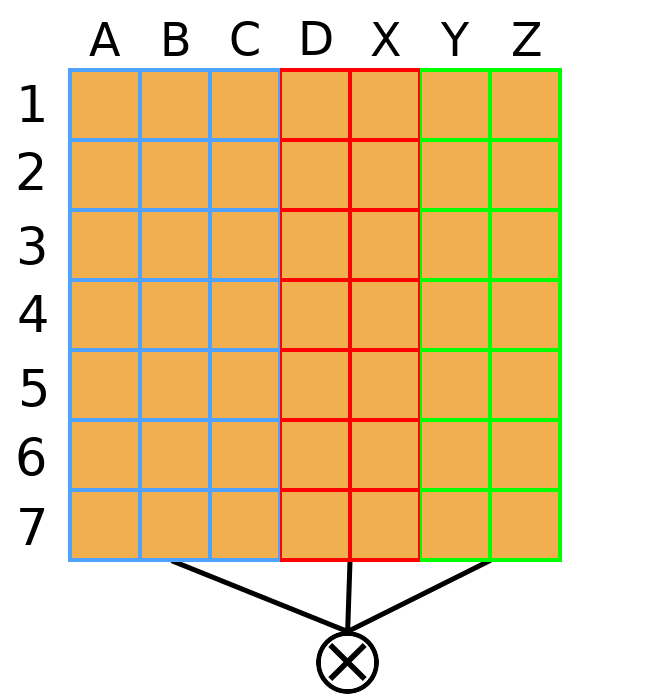
\includegraphics[height=0.25\textheight]{imgs/split-v.png}
  \end{figure}
  \begin{center}
    Partitions once greedily.
  \end{center}

  \textbf{Prometheus:}

  \begin{figure}
    \centering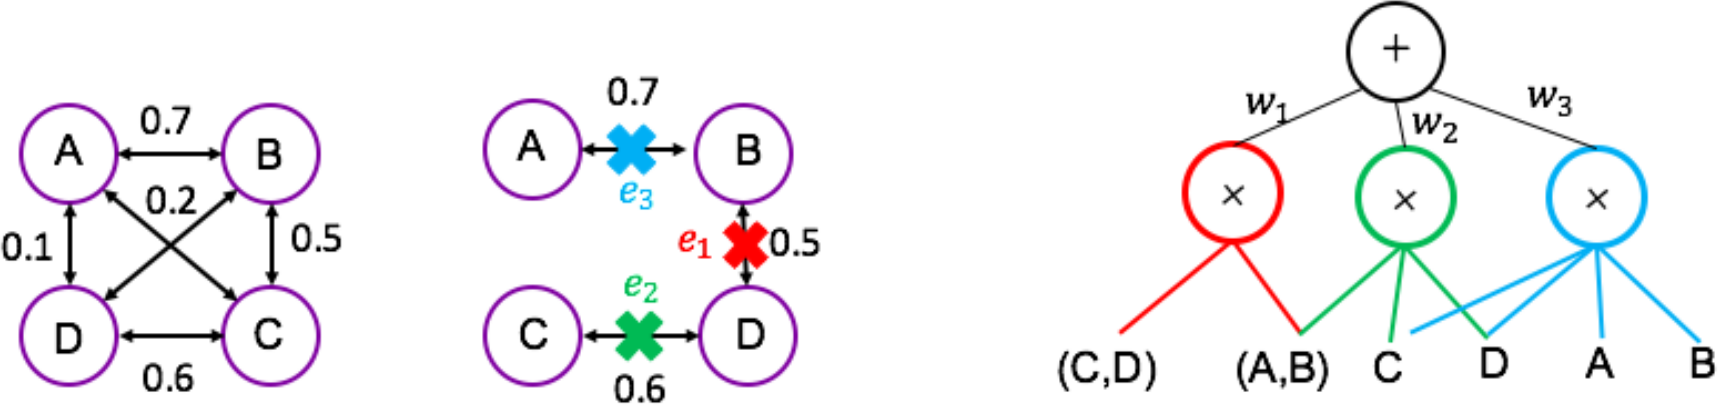
\includegraphics[height=0.25\textheight]{imgs/mst_decomp.png}
  \end{figure}
  \begin{center}
    Partitions by Maximum Spanning Tree and reuses repeated scopes.
  \end{center}
\end{frame}

\begin{frame}
  \frametitle{Maximum spanning trees (MSTs)}

  \begin{definition}[Minimum spanning tree]
    Let $G=(V,E)$ be an undirected weighted graph. The minimum spanning tree is the subgraph
    $T\subseteq G$ where $V_T=V_G$ and $E_T\subseteq E_G$ st $\sum_{e\in E_T} w_e$ is minimum,
    where $w_e$ is the weight associated with edge $e$.
  \end{definition}
  \vspace{0.25cm}

  \begin{figure}
    \centering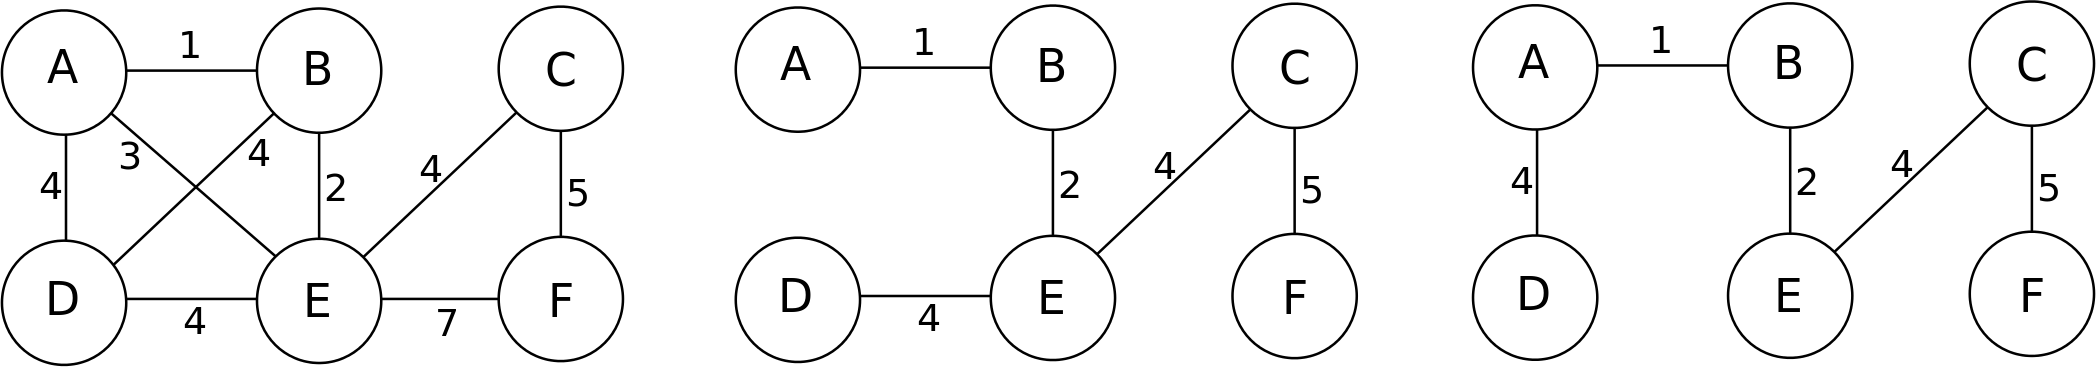
\includegraphics[width=\textwidth]{imgs/mst.png}
  \end{figure}

  \vspace{0.25cm}
  \small Maximum spanning tree $\equiv$ minimum spanning tree with negated weights
\end{frame}

\begin{frame}
  \frametitle{Graph partitioning}

  Let $S=\{X_1,X_2,\ldots,X_n\}$ be the scope and $D_S$ be the available data restricted to scope
  $S$. Let $G$ be a complete undirected weighted graph, where $V_G=S$, and each weight $w_{x,y}$ of
  edge $e=\{x,y\}\in E_G$ is defined by the Pearson correlation between the two variables $x$ and
  $y$:
  \vspace{0.125cm}

  \begin{equation*}
    w_{x,y} = \frac{\sum_{i=1}^n (x_i-\overline{x})(y_i-\overline{y})}{\sqrt{\sum_{i=1}^n (x_i-
    \overline{x})^2}\sqrt{\sum_{i=1}^n (y_i-\overline{y})^2}}
  \end{equation*}
  \vspace{0.125cm}

  \begin{block}{What we want}
    Partition $S$ in such a way that each subset has high correlation between their variables.
  \end{block}
\end{frame}

\begin{frame}
  \frametitle{Prometheus}

  \begin{block}{Their (\cite{prometheus}) proposal:}
    Let $T$ be $G$'s maximum spanning tree. Remove the weakest edge from $T$. The components of the
    resulting graph are the different partitions. Add these partitions to a list $L$ and repeat
    until there are no edges left to remove.
  \end{block}

  \begin{figure}
    \centering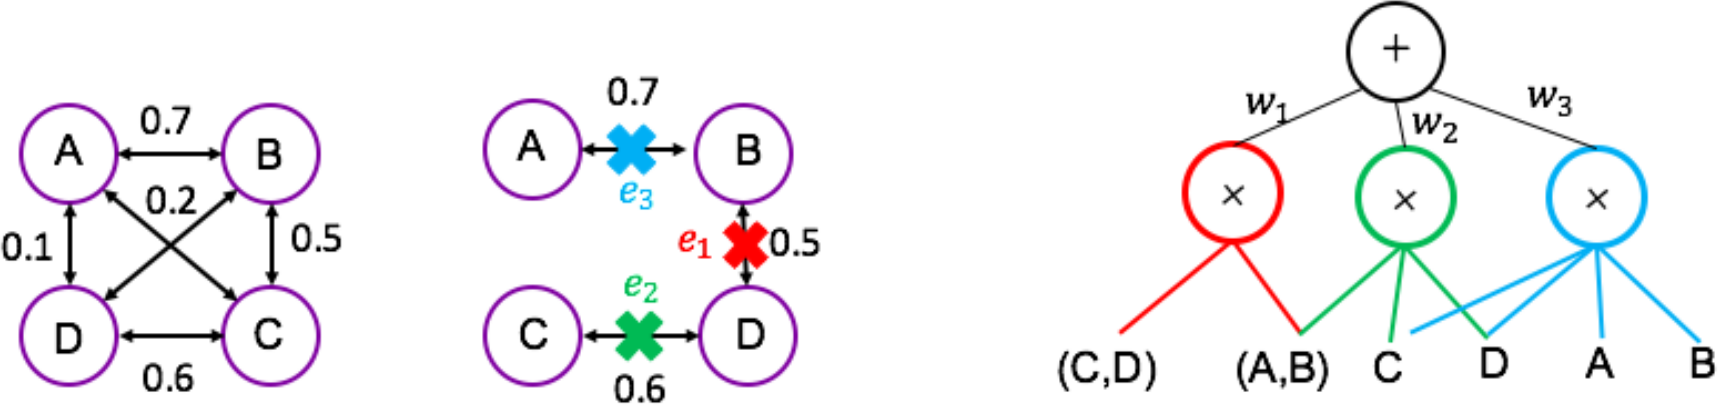
\includegraphics[width=\textwidth]{imgs/mst_decomp.png}
  \end{figure}

  Each element in $L$ is a product decomposition between the partitioned scopes. If such a
  sub-scope already exists, reuse.
\end{frame}

\begin{frame}
  \frametitle{The problem}

  An MST could potentially discard highly correlated pairs of variables.

  \begin{figure}
    \centering
    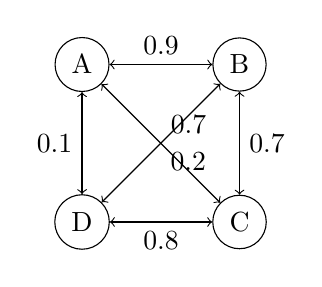
\begin{tikzpicture}
      \node[shape=circle,draw=black] (D) at (0, 0) {D};
      \node[shape=circle,draw=black] (C) at (2, 0) {C};
      \node[shape=circle,draw=black] (A) at (0, 2) {A};
      \node[shape=circle,draw=black] (B) at (2, 2) {B};
      %\begin{scope}[every node/.style={fill=white,circle}]
      \path[<->] (A) edge node[above] {$0.9$} (B);
      \path[<->] (A) edge node[below right] {$0.2$} (C);
      \path[<->] (A) edge node[left] {$0.1$} (D);
      \path[<->] (B) edge node[above right] {$0.7$} (D);
      \path[<->] (B) edge node[right] {$0.7$} (C);
      \path[<->] (C) edge node[below] {$0.8$} (D);
      %\end{scope}
    \end{tikzpicture}
    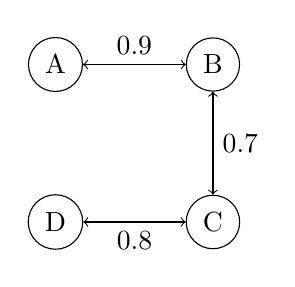
\begin{tikzpicture}
      \node[shape=circle,draw=black] (D) at (0, 0) {D};
      \node[shape=circle,draw=black] (C) at (2, 0) {C};
      \node[shape=circle,draw=black] (A) at (0, 2) {A};
      \node[shape=circle,draw=black] (B) at (2, 2) {B};
      \path[<->] (A) edge node[above] {$0.9$} (B);
      \path[<->] (B) edge node[right] {$0.7$} (C);
      \path[<->] (C) edge node[below] {$0.8$} (D);
    \end{tikzpicture}
  \end{figure}

  The above graph would generate the same SPN as the last example, and completely discard B and D's
  high-correlation interaction.
\end{frame}

\begin{frame}
  \frametitle{Our (initial) idea}

  Instead of partitioning by MST, try other graph partitioning methods.

  \begin{block}{Max-flow min-cut}
    Given two vertices $s$ and $t$, the max-flow problem describes a minimum cut that completely
    disconnects $s$ from $t$.
  \end{block}
  \begin{alertblock}{Problem:}
    How to choose $s$ and $t$? Should $\{s,t\}\subset S$? Different choices could favor certain
    variables. Should $s$ and $t$ be artificial nodes? If so, should $s$ and $t$ connect to all
    other vertices in $S$? In this case, either $(s,v)\in E_G$, $\forall v\in S$; or $(v,t)\in E_G$
    is a cut. So should $s$ and $t$ only connect to certain nodes? We fall into the same problem of
    favoring certain variables.
  \end{alertblock}
  \vspace{0.25cm}

  \textbf{Too many problems! Try something else?}
\end{frame}

\begin{frame}
  \frametitle{Our (current) idea}

  Graph partitioning is NP-hard, but we can try a heuristic algorithm.

  \begin{block}{Kernighan-Lin algorithm}
    Bipartition a graph $G$ into two subsets of fixed size $X$ and $Y$ by greedily minimizing the
    sum of weights that go from $X$ to $Y$ and vice-versa.
  \end{block}
  \begin{alertblock}{Problem:}
    If we only consider balanced partitions, the algorithm is fast, but the resulting SPN might be
    too simple. If we consider partitions of arbitrary lengths, then we have to try every possible
    bipartition of size in range $[1,\lfloor\frac{|S|}{2}\rfloor]$.
  \end{alertblock}
  \vspace{0.25cm}

  \textbf{Ideas?}
\end{frame}

\begin{frame}
  \frametitle{Parameter learning}

  \begin{table}[h]
    \centering
    \begin{tabular}{c}
      \hline
      \multicolumn{1}{c}{\bfseries Partial derivatives wrt internal node $j$}\\
      \hline\\
      \(\displaystyle \ddspn{S}{S_j}=\sum_{\substack{n\in\Pa(j)\\n:\text{ sum}}}w_{n,j}
        \ddspn{S}{S_n}+\sum_{\substack{n\in\Pa(j)\\n:\text{ product}}}\ddspn{S}{S_n}\prod_{k\in\Ch(n)
        \setminus\{j\}}S_k\) \\~\\
      \hline
      \multicolumn{1}{c}{\bfseries Partial derivatives wrt weight $w_{n,j}$}\\
      \hline\\
      \(\displaystyle \ddspn{S}{w_{n,j}} = S_j\ddspn{S}{S_n} \) \\~\\
      \hline
    \end{tabular}
  \end{table}
\end{frame}

\begin{frame}
  \frametitle{Gradient descent}

  \textbf{Recapping gradient descent:}
  \vspace{0.125cm}

  \begin{table}[t]
    \centering
    \begin{tabular}{rc}
      \toprule
      \rowcolor{Yellow}
      \textbf{\textsc{Generative}} & \\  \rowcolor{Cyan}
      \textbf{Soft} & \(\displaystyle \Delta w_{n,j}=\eta\ddspn{S(\mathbf{x}, \mathbf{y})}{w_{n,j}}\) \\
      \rowcolor{Cyan}
      \textbf{Hard} & \(\displaystyle \Delta w_{n,j}=\eta\frac{c_{n,j}}{w_{n,j}}\) \\
      \rowcolor{Yellow}
      \textbf{\textsc{Discriminative}} &  \\
      \rowcolor{Cyan}
      \textbf{Soft} & \(\displaystyle \Delta
        w_{n,j}=\eta\left(\frac{1}{S(\mathbf{y},\mathbf{x})}\ddspn{S(\mathbf{y},\mathbf{x})}{w_{n,j}}-\frac{1}{S(\mathbf{x})}
        \ddspn{S(\mathbf{x})}{w_{n,j}}\right)\) \\
      \rowcolor{Cyan}
      \textbf{Hard} & \(\displaystyle \Delta w_{n,j}=\eta\frac{\Delta c_{n,j}}{w_{n,j}}\) \\
      \bottomrule
    \end{tabular}
  \end{table}
  \vspace{0.125cm}

  Can we do something different (perhaps better)?
\end{frame}

\begin{frame}
  \frametitle{A Unified Approach for Learning the Parameters of Sum-Product Networks}

  \begin{figure}
    \centering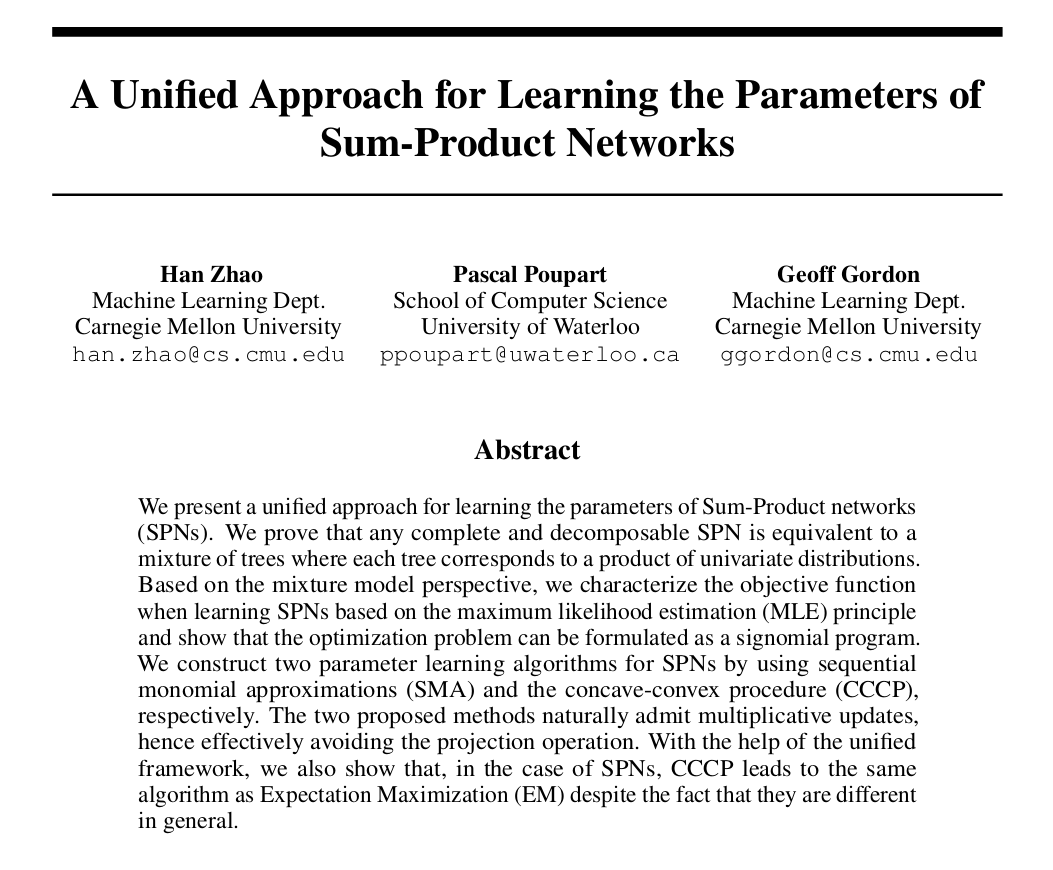
\includegraphics[height=0.7\textheight]{imgs/unified.png}
  \end{figure}
\end{frame}

\begin{frame}
  \frametitle{A Unified Approach for Learning the Parameters of Sum-Product Networks}

  \cite{unified} show (amongst other things) that:
  \begin{itemize}
    \item Expectation-Maximization (EM) is equivalent to Concave-Convex Procedure (CCCP);
    \item CCCP is empirically better than (some other) methods;
    \item CCCP also converges faster;
    \item A simple structure + CCCP is able to achieve better results than a more complex structure
      with no parameter learning.
  \end{itemize}
\end{frame}

\begin{frame}
  \frametitle{Concave-Convex Procedure (CCCP)}

  \begin{theorem}[\cite{cccp}]
    Let $E(\vec{x})$ be an energy function with bounded Hessian $\frac{\partial^2
    E(\vec{x})}{\partial\vec{x}\partial\vec{y}}$. Then we can
    always decompose it into the sum of a convex function and a concave function.
  \end{theorem}

  \begin{theorem}[CCCP, \cite{cccp}]
    Consider an energy function $E(\vec{x})$ of form $E(\vec{x}) =
    E_{vex}(\vec{x})+E_{cave}(\vec{x})$ where $E_{vex}(\vec{x})$,
    $E_{cave}(\vec{x})$ are convex and concave functions of $\vec{x}$
    respectively. Then the discrete iterative CCCP algorithm $\vec{x}^t\mapsto
    \vec{x}^{t+1}$ given by:
    \begin{equation*}
      \vec{\nabla}E_{vex}\left(\vec{x}^{t+1}\right)=-\vec{\nabla}E_{cave}\left(\vec{x}^t\right)
    \end{equation*}
    is guaranteed to monotonically decrease the energy $E(\vec{x})$ as a function of
    time and hence to a minimum or saddle point of $E(\vec{x})$.
  \end{theorem}
\end{frame}

\begin{frame}
  \frametitle{CCCP for SPN parameter learning}

  CCCP weight update formula, which is equivalent to EM's:
  \vspace{0.125cm}

  \begin{equation*}
    w_{ij} \gets w_{ij} \frac{\partial S}{\partial S_i}(\mathbf{x})\frac{S_j(\mathbf{x})}{S(\mathbf{x})}
  \end{equation*}
  \vspace{0.125cm}

  where $j$ is a child node of $i$.
  \vspace{0.25cm}

  \begin{itemize}
    \item $\frac{\partial S}{\partial S_i}(\mathbf{x})$: partial derivative of the SPN $S$ wrt
      sub-SPN $S_i$ (i.e. the SPN rooted at $i$);
    \item $S_j(\mathbf{x})$: the value of $S_j$ given evidence $\mathbf{x}$;
    \item $S(\mathbf{x})$: value of root SPN $S$.
  \end{itemize}
\end{frame}

\begin{frame}[t,allowframebreaks]
  \frametitle{References}
  \printbibliography[heading=none]
\end{frame}

\end{document}
